\section{The applications: further results}
\label{sec:supp-app}

\subsection*{Prediction and structure}

Table~\ref{tab:app-prediction} gives, for the two applications, the root mean
squared error on the held-out weeks, its mean over the 20 partitions with the
standard error of \citet{Nadeau-Bengio-2003}, which corrects for the overlap
of the training samples, the ratio to the better of the two splines in each
partition, and the paired difference to the spline with the smaller mean
error, with the fraction of partitions in which it is negative.
Table~\ref{tab:app-structure} gives, for every block, the frequency with
which each method keeps it over the partitions, and
Table~\ref{tab:app-tuning} the choices of $J$, the penalty, the threshold
and $k$.

At Marylebone Road the comparison is that of Section 6.3 of the paper; the
constant coefficients have an error of 15.48~ppb, about a third more than
the methods with varying coefficients. At Dongsi the WAFC is ahead of the
spline fitted by REML, the better of the two splines in every partition, in
all 20 partitions and with either threshold, with an error smaller by 8\% on
average and a paired difference of $-0.070$ (standard error 0.023). There
both thresholds and both splines keep every block in the fit to the whole
sample, and the one standard error rule drops the pressure along the day of
the year in one partition and along the humidity in two.

Both splines choose $k = 80$, the top of the grid, in all 21 fits of each
application, and \texttt{k.check} flags two of the four smooths at
Marylebone Road in every fit and four to eight of the eight at Dongsi. The
WAFC chooses $J = 8$, the top of its grid, in the fit to the whole sample at
Marylebone Road and $J = 5$ or 6 in the partitions; at Dongsi it chooses
$J = 4$ in the fit to the whole sample and in 19 of the 20 partitions, and
every coefficient of a block it keeps is nonzero. At Marylebone Road,
extending the grids does not change the comparison: with $k$ up to 160 in
the first three partitions, REML and GCV again choose the largest dimension
and the error on the held-out weeks rises by about 3 to 4 percent, and in the
fit to the whole sample the cross-validated error of the WAFC at $J = 9$ is
larger than at $J = 8$. At Dongsi, where the splines also choose $k = 80$,
the grids were not extended.

% tables/app-prediction.tex -- tabela do supp_5.tex, Secao S10 (E5h, 2026-10-06; D21: cada tabela num
% \input proprio). So o lugar: o conteudo vem da E6.2 (os prediction-<app>.csv do compendio).
% E5k (2026-10-08): os numeros de results/tables/prediction-<app>.csv (o compendio e
% a verdade): rmse; se * nb_factor (o erro-padrao corrigido de Nadeau e Bengio, com o
% fator que o application_prediction() aplica a diferenca); ratio_best_spline; diff e
% diff_se_nb contra a coluna versus (gam.reml nas duas bases); wins (a fracao de
% particoes com erro abaixo do gam.reml, nao do melhor spline de cada particao, que
% so coincidem na beijing.heat, onde o gam.reml e o melhor em todas); r2. A legenda
% diz isso no lugar do "fraction of partitions in which a method beats that spline" da
% E5h. \color{colR1} dentro do float (D75(d)).
\begin{table}[tp]
\caption{The two applications, prediction on the held-out weeks over 20
partitions: the root mean squared error (RMSE), mean and standard error with
the correction of \citet{Nadeau-Bengio-2003}; its ratio to that of the better
of the two splines in each partition; the paired difference to the spline
with the smaller mean error, GAM (REML) in both applications, with the
corrected standard error, and the fraction of partitions in which it is
negative; and $R^2$, one minus the ratio of the mean squared error to the
variance of the held-out response. WAFC: the threshold of the one standard
error rule; WAFC (cv threshold): the threshold of the smallest
cross-validated error.}
\label{tab:app-prediction}
\centering
\small
\begin{tabular}{lccccc}
\hline
 & RMSE & Ratio & Difference & Negative & $R^2$ \\
\hline
\multicolumn{6}{l}{Marylebone Road, total oxidant (ppb)} \\
WAFC & 11.75 (0.28) & 1.025 & 0.28 (0.22) & 0.30 & 0.68 \\
WAFC (cv threshold) & 11.52 (0.32) & 1.005 & 0.05 (0.11) & 0.40 & 0.69 \\
GAM (REML) & 11.47 (0.32) & 1.000 & -- & -- & 0.69 \\
GAM (GCV) & 11.49 (0.33) & 1.002 & 0.02 (0.02) & 0.10 & 0.69 \\
Constant coefficients & 15.48 (0.30) & 1.352 & 4.02 (0.30) & 0.00 & 0.44 \\
\hline
\multicolumn{6}{l}{Dongsi, logarithm of PM2.5} \\
WAFC & 0.800 (0.017) & 0.920 & $-$0.070 (0.023) & 1.00 & 0.53 \\
WAFC (cv threshold) & 0.797 (0.016) & 0.916 & $-$0.074 (0.021) & 1.00 & 0.54 \\
GAM (REML) & 0.871 (0.027) & 1.000 & -- & -- & 0.45 \\
GAM (GCV) & 0.892 (0.029) & 1.024 & 0.021 (0.006) & 0.00 & 0.42 \\
Constant coefficients & 1.059 (0.016) & 1.218 & 0.188 (0.026) & 0.00 & 0.18 \\
\hline
\end{tabular}
\end{table}

% tables/app-structure.tex -- tabela do supp_5.tex, Secao S10 (E5h, 2026-10-06; D21: cada tabela num
% \input proprio). So o lugar: o conteudo vem da E6.2 (os structure-<app>.csv e choices-<app>.csv do compendio).
% E5k (2026-10-08): os numeros de results/tables/ (o compendio e a verdade). Painel (a),
% do structure-<app>.csv: kept_<rotulo> * 20 e, entre parenteses, range_<rotulo> (a
% amplitude no ajuste inteiro nos pontos desenhados, D75(b); zero quando full_<rotulo> e
% FALSE). O painel (b) das escolhas foi a tables/app-tuning.tex (Table S7): as duas
% juntas, em espaco duplo, passavam 454 pt da pagina. \color{colR1} dentro do float (D75(d)).
\begin{table}[tp]
\caption{The two applications, structure: for every block, the number of the
20 partitions in which each method keeps it and, in parentheses, the range of
the component in the fit to the whole sample over the points drawn in
Figure~2 of the paper and Figure~\ref{fig:beijing}, which is zero when that
fit drops the block; in ppb for the background and in percentage points for
the slope at Marylebone Road, and in the logarithm of PM2.5 at Dongsi, per
unit of the covariate (m/s, $^{\circ}$C, hPa) for the coefficients. WAFC
(cv): the threshold of the smallest cross-validated error.}
\label{tab:app-structure}
\centering
\small
\setlength{\tabcolsep}{5pt}
\begin{tabular}{lcccc}
\hline
Block & WAFC & WAFC (cv) & GAM (REML) & GAM (GCV) \\
\hline
\multicolumn{5}{l}{Marylebone Road} \\
Background, date & 20 (24.2) & 20 (24.2) & 20 (22.9) & 20 (24.4) \\
Background, wind speed & 12 (0) & 20 (5.75) & 20 (7.82) & 20 (7.38) \\
Slope on NOx, date & 20 (15.8) & 20 (15.8) & 20 (20.8) & 20 (21.0) \\
Slope on NOx, wind speed & 0 (0) & 19 (0.795) & 18 (1.15) & 19 (1.78) \\
\hline
\multicolumn{5}{l}{Dongsi} \\
Level, day of the year & 20 (6.33) & 20 (6.33) & 20 (8.36) & 20 (8.89) \\
Level, humidity & 20 (2.26) & 20 (2.26) & 20 (2.15) & 20 (2.10) \\
Wind speed, day of the year & 20 (0.417) & 20 (0.417) & 20 (0.685) & 20 (0.744) \\
Wind speed, humidity & 20 (0.294) & 20 (0.294) & 20 (0.211) & 20 (0.212) \\
Temperature, day of the year & 20 (0.101) & 20 (0.101) & 20 (0.178) & 20 (0.198) \\
Temperature, humidity & 20 (0.0735) & 20 (0.0735) & 20 (0.0654) & 20 (0.0663) \\
Pressure, day of the year & 19 (0.109) & 20 (0.109) & 20 (0.186) & 20 (0.221) \\
Pressure, humidity & 18 (0.0501) & 20 (0.0501) & 20 (0.0350) & 20 (0.0358) \\
\hline
\end{tabular}
\end{table}

% tables/app-tuning_6.tex -- a Table S7 da k = 6 (E5b, 2026-10-12): a de app-tuning.tex com as
% tres linhas do tempo por ajuste (pergunta 68(i)), da coluna time de
% results/tables/choices-<app>.csv, em segundos: split 0 e a mediana (minimo--maximo) dos
% splits 1 a 20; o WAFC e a linha wafc.cv1se (o wafc.cv e o mesmo ajuste). As aplicacoes
% rodaram no notebook (i7-10875H), uma unidade por nucleo (E6.2).
% Cabecalho de app-tuning.tex: tabela do supp_5.tex, Secao S10 (E5k, 2026-10-08; D21: cada tabela
% num \input proprio). O painel (b) da Table S6 da E5h ("the choices of J, lambda, the
% threshold and k"), separado porque as duas juntas passavam 454 pt da pagina em espaco
% duplo. Os numeros de results/tables/choices-<app>.csv (o compendio e a verdade): split 0
% e a mediana (minimo--maximo) dos splits 1 a 20 de J e lambda (iguais nas duas linhas do
% WAFC), t_frac * 100 (o limiar como fracao da maior norma de bloco do ajuste, a coluna c
% do wafc_threshold()), nzero, k (o mesmo nas duas moduladoras, "80,80", k_top TRUE nos
% 21 ajustes) e kcheck_n_low (de 4 suavizacoes em marylebone, 8 na beijing.heat; os dois
% splines dao os mesmos resumos, por isso uma linha so). \color{colR1} dentro do float (D75(d)).
\begin{table}[tp]
\caption{The two applications, tuning: the choices in the fit to the whole
sample and their median (range) over the 20 partitions. $J$ and $\pen$ are
those of the WAFC, which the two thresholds share; the threshold is in
percent of the largest block norm of the fit, followed by the number of
nonzero coefficients after it; $k$ is the dimension chosen by the two
splines, at both modulators, and the  row
of smooths flagged the number of smooths that
\texttt{k.check} of \texttt{mgcv} flags, of 4 at Marylebone Road and of 8 at
Dongsi, which is the same for REML and GCV. The grids are
$J \in \{2,\dots,8\}$ and $k \in \{5,10,20,40,80\}$. The time is that of
one fit with its tuning, in seconds on one core of an Intel Core i7-10875H.}
\label{tab:app-tuning}
\centering
\small
\begin{tabular}{lcccc}
\hline
 & \multicolumn{2}{c}{Marylebone Road} & \multicolumn{2}{c}{Dongsi} \\
 & Whole & Partitions & Whole & Partitions \\
\hline
$J$ & 8 & 5 (5--6) & 4 & 4 (3--4) \\
$\pen \times 10^{3}$ & 101.9 & 40.2 (29.7--73.2) & 0.43 & 0.88 (0.56--1.60) \\
\multicolumn{5}{l}{WAFC} \\
\quad Threshold (\%) & 77 & 77 (56--93) & 0.95 & 0.98 (0.55--1.13) \\
\quad Nonzero coefficients & 458 & 77 (62--152) & 120 & 120 (56--120) \\
\multicolumn{5}{l}{WAFC (cv threshold)} \\
\quad Threshold (\%) & 5.7 & 10.6 (3.9--33.3) & 0.46 & 0.46 (0.28--1.02) \\
\quad Nonzero coefficients & 488 & 108 (77--178) & 120 & 120 (56--120) \\
\multicolumn{5}{l}{GAM (REML) and GAM (GCV)} \\
\quad $k$ & 80 & 80 (80--80) & 80 & 80 (80--80) \\
\quad Smooths flagged & 2 & 2 (2--2) & 4 & 4 (4--8) \\
\multicolumn{5}{l}{Time per fit (s)} \\
\quad WAFC & 2163 & 2387 (1764--3546) & 8830 & 7355 (6420--7909) \\
\quad GAM (REML) & 9.2 & 7.1 (6.9--7.4) & 27.6 & 23.4 (22.5--25.9) \\
\quad GAM (GCV) & 202 & 150 (143--152) & 474 & 424 (359--461) \\
\hline
\end{tabular}
\end{table}


\subsection*{Beijing}

The data are the hourly observations at the site Dongsi of the Beijing
Multi-Site Air Quality data of the UCI Machine Learning Repository
\citep{Chen-UCI-2017}, from 1 March 2013 to 28 February 2017, under the
attribution given in the Acknowledgements of the paper. Dongsi is one of
the 12 nationally controlled sites of the data set, which are among the 36
sites whose PM2.5 series \citet{Zhang-Guo-Dong-He-Xu-Chen-2017} analyze;
the meteorological variables of a site are those of the nearest station of
the China Meteorological Administration, which for Dongsi changes in
February 2015 \citep[Table~S1 of their Supplementary
Material]{Zhang-Guo-Dong-He-Xu-Chen-2017}. The 34,287 hours with PM2.5,
temperature, pressure, dew point and wind speed observed, a relative humidity in $(0,100]$
and a positive PM2.5 are used. The response is the logarithm of PM2.5, the
linear covariates are the constant, the wind speed (m/s), the temperature
($^{\circ}$C) and the pressure minus 1000 hPa, and the modulators are the day
of the year, from 0 on 1 January with the hour as a fraction of the day, and
the relative humidity (\%), computed from the temperature and the dew point by
the Magnus formula; every coefficient is modulated by both, so that $p = 4$,
$q = 2$ and the model has eight blocks. The day of the year is periodic, as
the periodized basis is. The splits, the methods and their tuning are those
of Section 6 of the paper.

The winter heating season of Beijing and the North China Plain usually runs
from 15 November to 15 March, and the weather-adjusted PM2.5 level rises
significantly at its start and falls at its end in every season from 2010 to
2014 \citep[Section~7]{Liang-Zou-Guo-Li-Zhang-Zhang-Huang-Chen-2015}; the
effective dates move with the temperature (for instance, the season started
on 3 November in 2012), so the marks at 15 November and 15 March in
Figure~\ref{fig:beijing} are nominal. Along the day of the year, the mean of
the component of a coefficient inside the nominal season minus its mean
outside it is, in the fit of the WAFC to the whole sample, $-0.18$ per m/s
for the wind speed ($-0.19$ to $-0.13$ over the partitions), $-0.056$ per
$^{\circ}$C for the temperature ($-0.058$ to $-0.031$) and $-0.028$ per hPa
for the pressure ($-0.032$ to 0), and the two splines give $-0.17$ to
$-0.18$, $-0.062$ and $-0.033$. The three differences are negative in every
fit of the WAFC and of the two splines, except that of the pressure in the
partition in which the WAFC drops that block: inside the season a unit of
wind speed goes with a larger decrease of PM2.5, and a degree of temperature
with a smaller increase, than outside it.

% figures/app-beijing.tex -- Figure S1 do supp_5.tex, Secao S10 (E5h, 2026-10-06;
% D21, D57). A figura e a beijing.heat.pdf do compendio (R/application_report.R).
% Duas escolhas de apresentacao da E5h, a confirmar na E5b: (i) a linha do nivel
% (o intercepto a vento zero, 0 C e 1000 hPa) nao e desenhada (D67(f)), o que pede
% tirar a linha `one` da figura no compendio; (ii) a borda da umidade se decide
% depois da rodada (D67(e)). As marcas da temporada sao as nominais (D66).
% E5k (2026-10-08): a caixa virou a figura, copia de results/figures/beijing.heat.pdf
% (refeita depois do piloto: o rug, D75(e), e a umidade cortada a ~15% e ~95%,
% `trim: rh: [6, 4]` do application.yaml, D67(e)). A figura do compendio ainda tem a
% linha do nivel; ate o compendio ter a opcao sem ela (handoff-E5k.md), o recorte
% abaixo a tira sem mexer no PDF: a faixa da legenda (do topo ate 22 bp) e as tres
% linhas de baixo (de 218 bp ate o fim), na pagina de 518 x 806 bp do PDF; as duas
% medidas caem em faixas brancas (pdftoppm a 72 dpi). Quando o compendio tirar a
% linha, volta a um \includegraphics so. A legenda segue a da Figure 2 (D68(g), E5j):
% os tipos de linha saem (a legenda do PDF os nomeia), "band" no lugar de "grey", os
% cortes ditos; o achado fica no texto da S10, como o da Figure 2 no 6.3 (a legenda com
% ele passava 98 pt da pagina). \color{colR1} dentro do float (D75(d)).
\begin{figure}[tp]
\centering
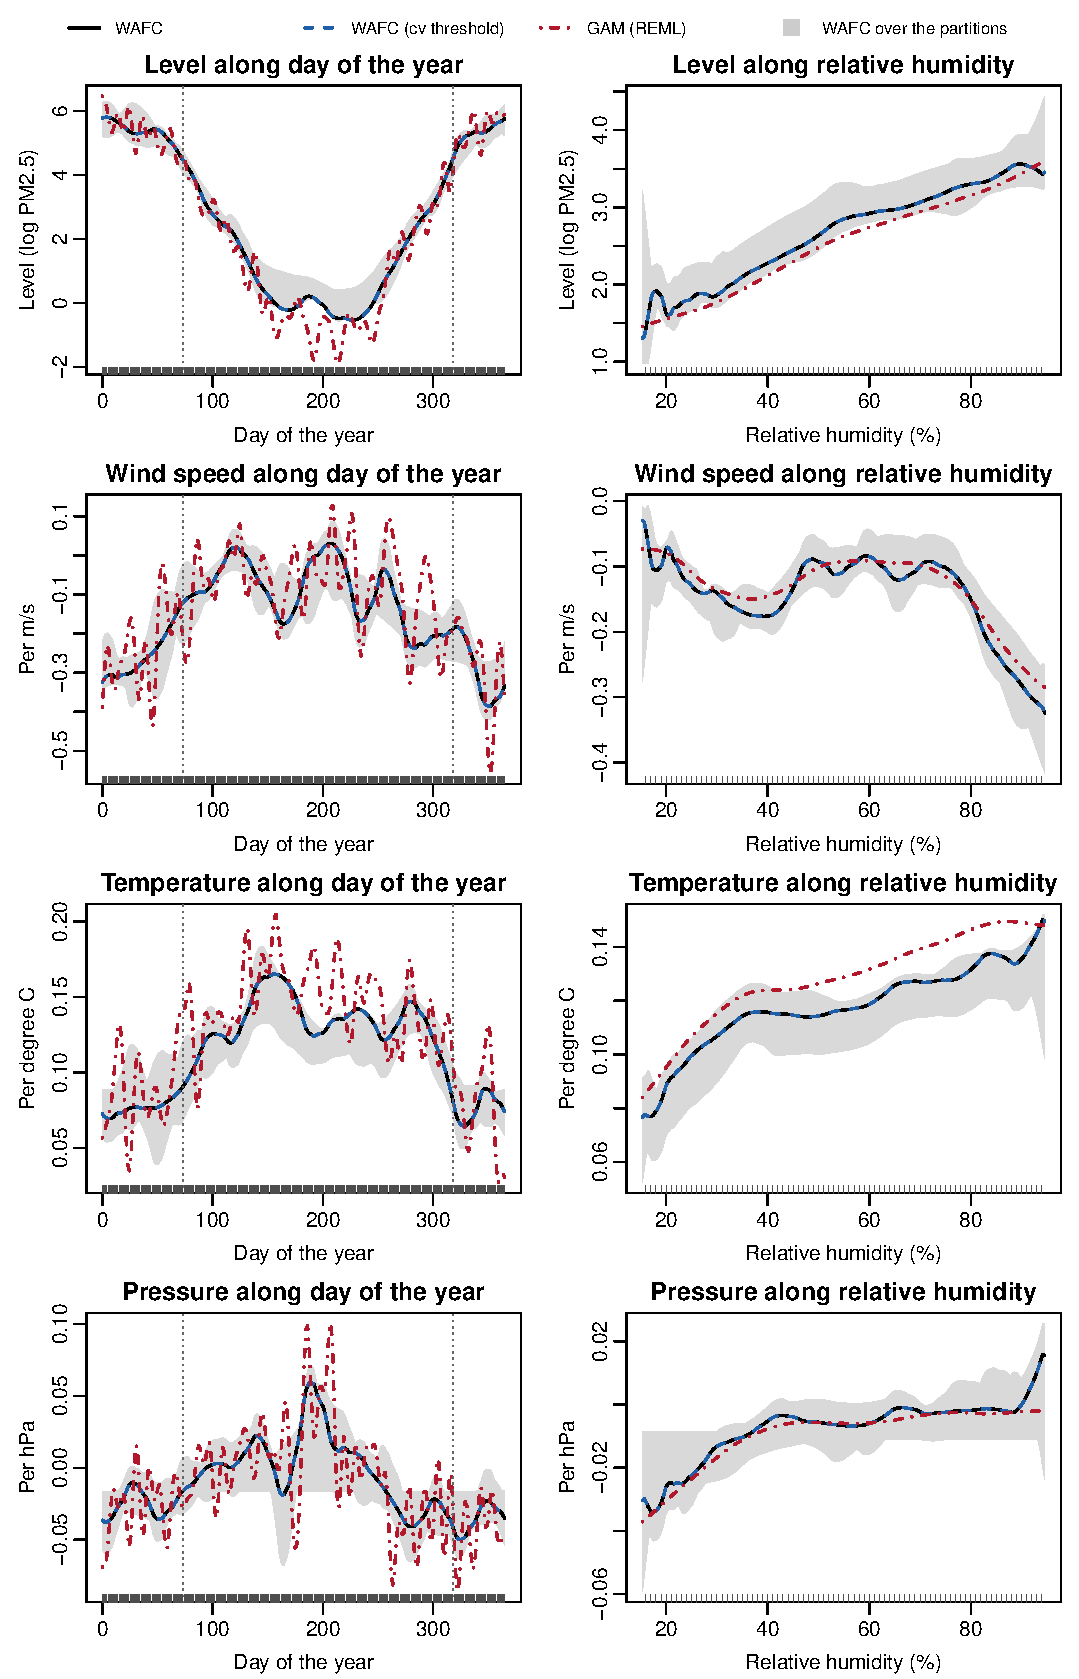
\includegraphics[width=0.72\textwidth,trim=0 784 0 0,clip]{figures/beijing.heat.pdf}\\
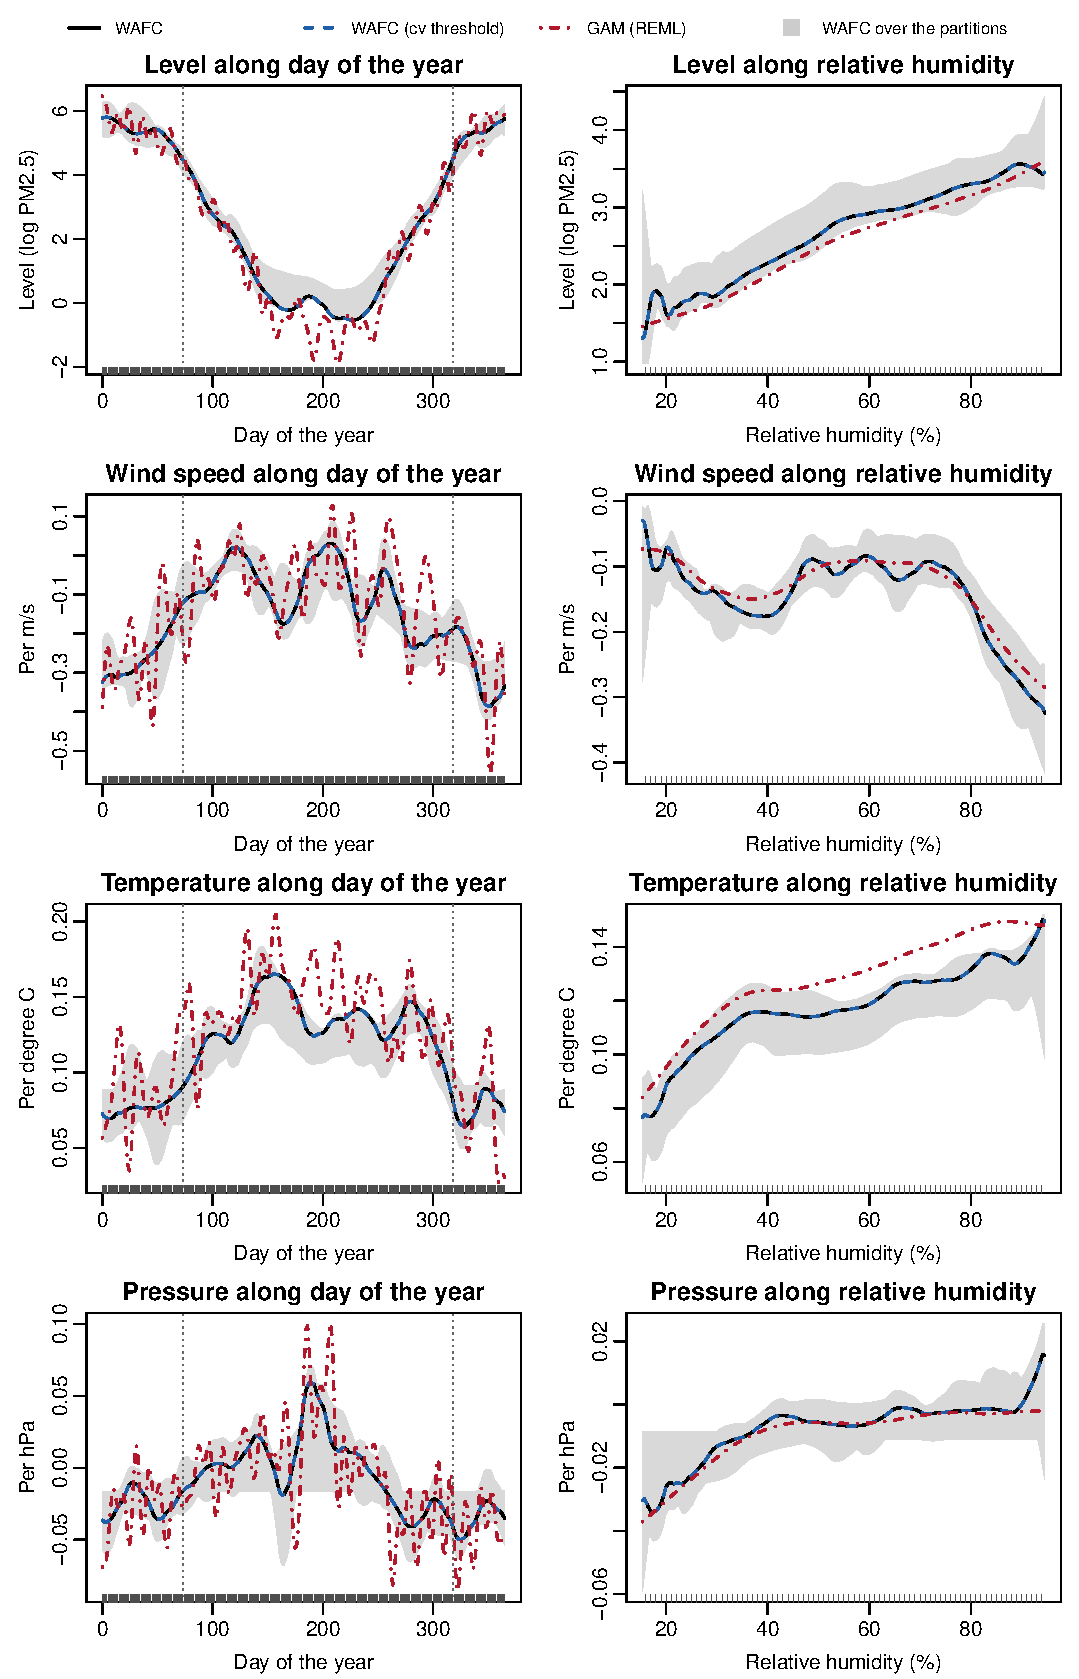
\includegraphics[width=0.72\textwidth,trim=0 0 0 218,clip]{figures/beijing.heat.pdf}
\caption{Beijing, Dongsi, hourly, March 2013 to February 2017: the
coefficients of the wind speed (top, per m/s), the temperature (middle, per
$^{\circ}$C) and the pressure (bottom, per hPa) for the logarithm of PM2.5,
along the day of the year (left) and the relative humidity (right), with the
component of the other modulator at its sample mean; the band is the range
of the WAFC over 20 fits on 70\% of the weeks, and the vertical lines mark
the nominal heating season, 15 November to 15 March. Not shown: the level,
which moves along the year with the coefficient of the temperature, and the
relative humidity below about 15\% and above about 95\%, where the
periodized basis joins the two ends of its range; ticks on the axes mark the
observed values.}
\label{fig:beijing}
\end{figure}

% E5h: a figura S1 cai depois das referencias sem isto.
\clearpage


%%%%%%%%%%%%%%%%%%%%%%%%%%%%%%%%%%%%%%%%%%%%%%%%%%%%%%%%%%%%%%%%%%%%%%%%%%%%%%
\bibhang=1.7pc
\bibsep=2pt
\fontsize{9}{14pt plus.8pt minus .6pt}\selectfont
\renewcommand\bibname{\large \bf References}
